% Converted from ANTARA_MCR_first draft.docx. Numbers and claims remain unverified.
\section{Mission Context, Objectives, and Success Criteria}\label{executive-summary-document-purpose-and-scope}

\subsection{Executive Summary}\label{executive-summary}

Project ANTARA is a 3U CubeSat mission at BITS Pilani, K.K. Birla Goa
Campus, dedicated to the in-situ characterization of the South Atlantic
Anomaly (SAA) radiation environment. Operating in a 600 km
Sun-Synchronous Orbit (97.6° inclination), the spacecraft carries a
custom Flux Particle Detector Unit (FPDU) payload to measure
unidirectional differential proton flux across the 5--100 MeV range in
a proposed multi-channel energy reconstruction.

The mission is structured around three tiers of success that scale
spatial resolution, coverage, and scientific ambition. Beyond its
scientific objective, ANTARA serves as a student satellite training
platform, exposing undergraduate students to the complete spacecraft
development lifecycle from concept through operations.

This document represents the Mission Concept Review (MCR) package for
Project ANTARA, consolidating mission requirements, architecture, orbit
design, operational concept, subsystem design status, and simulation
results.

\subsection{Mission Need}\label{mission-need}

The ANTARA mission has been conceptualized to address a combination of
scientific, educational, and national-level needs associated with the
growing importance of space-based radiation studies and indigenous
small-satellite development. Modern spacecraft operating in Low Earth
Orbit (LEO) are increasingly exposed to harsh radiation environments
that can significantly affect mission reliability, onboard electronics,
detector systems, and long-term spacecraft survivability. Among these
environments, the South Atlantic Anomaly (SAA) represents one of the
most severe and scientifically significant radiation regions encountered
by satellites in LEO.

\begin{figure}[htbp]\centering
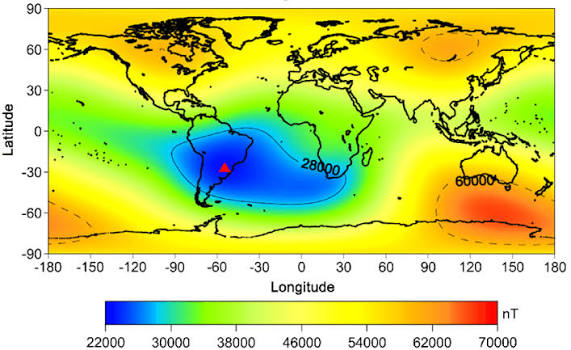
\includegraphics[width=\linewidth,height=0.65\textheight,keepaspectratio]{./media/saa_magnetic_anomaly.png}
\caption{South Atlantic Magnetic Anomaly (year 2000; source image from original draft).}\label{fig:saa-background}
\end{figure}

Although several trapped-radiation models such as AP8 and AP9 currently
exist, substantial uncertainties remain regarding temporal proton-flux
variability, storm-time behavior, directional anisotropies, and
localized radiation structures within the SAA. Existing models are
primarily statistical and often lack sufficient real-time data required
for modern small-satellite missions and future radiation-aware
spacecraft operations.

The ANTARA mission seeks to contribute toward closing these gaps through
direct in-situ measurement of high-energy proton populations using a
dedicated CubeSat operating in a Sun-Synchronous Orbit. The project also
enables students to gain practical experience in CubeSat designing and
modelling.


\subsubsection{Educational Motive}\label{educational-motive}One of the primary motivations behind ANTARA is the creation of an
educational and research platform capable of providing hands-on
experience in real-world spacecraft development.

The mission enables participating students to experience all major
phases of aerospace project development. Unlike isolated academic
laboratory experiments, CubeSat missions introduce students to highly
constrained engineering environments where mass, power, thermal limits
and others interact simultaneously. This systems-level complexity is one
of the most important educational benefits of the ANTARA mission.

\subsubsection{Scientific Motive}\label{scientific-motive}The primary scientific motivation behind ANTARA is the need for improved
understanding of the trapped proton environment within the South
Atlantic Anomaly and its implications for spacecraft operations,
radiation modelling, and near-Earth space science.

The South Atlantic Anomaly represents the region where the inner Van
Allen radiation belt approaches closest to Earth due to the offset and
tilt of Earth's magnetic dipole. Spacecraft traversing this region are
exposed to significantly elevated fluxes of energetic charged particles,
particularly high-energy protons capable of producing Single Event
Upsets (SEUs), sensor noise, detector saturation, memory corruption,
semiconductor degradation, and cumulative radiation damage.

ANTARA aims to contribute toward this scientific need by directly
measuring Unidirectional Differential Proton Flux (FPDU) within the
energy range of 5 MeV to 100 MeV using an onboard proton detection
payload. The mission seeks to generate spatially and temporally
correlated radiation datasets that can be compared against existing
radiation models including AP8 and AP9.

\subsubsection{National Motive}\label{national-motive}From a national perspective, ANTARA aligns strongly with India's growing
emphasis on indigenous space technology development, scientific
self-reliance, and advanced research capability. The mission contributes
toward India's requirement for indigenous expertise in spacecraft
systems engineering, radiation-aware electronics, mission operations,
and advanced satellite technologies.

Also, the satellites in the past few years have faced various anomalies
with this region due to which communication signals with them were lost.
Data collected by ANTARA maps the shifting borders of the SAA, allowing
Indian satellites to shield or power down domestic defense and
communication satellites before they sustain damage. ANTARA provides an
opportunity for low-cost effective and indigenous space tech to be
tested via its CubeSat.


\subsection{Mission Significance}\label{mission-significance}

\subsubsection{Primary Flight Objective}\label{primary-flight-objectives}
The primary objective is to measure and map unidirectional differential proton flux in the South Atlantic Anomaly over the 5--100~MeV range.

\subsubsection{Secondary Mission Objectives}\label{b.-secondary-mission-objectives}
The secondary objectives are to examine East--West asymmetry, characterize the bifurcation of the SAA, investigate atmospheric-loss coupling, and develop corrections to radiation-model predictions from ANTARA measurements. Storm-time comparisons remain an exploratory objective dependent on available observations. The detector architecture and channel definition remain under development; the science-success criteria are proposed targets to be tested against actual detection and sampling capability.

\subsection{Mission Success Criteria}\label{mission-success-criteria}

Mission success criteria define the measurable conditions under which
the ANTARA mission can be considered operationally and scientifically
successful. These criteria establish a structured framework for
evaluating mission performance at different levels of achievement
throughout the mission lifecycle. The criteria are divided into three
progressive categories:

\begin{itemize}
\item
  Minimum Mission Success (MMSC)
\item
  Full Mission Success (MSC)
\item
  Extended Mission Success (EMSC)
\end{itemize}

\subsubsection{Minimum Mission Success Criteria (MMSC)}\label{minimum-mission-success-criteria-mmsc}The MMSC defines the lowest acceptable bar for declaring the mission a
scientific and engineering success. Meeting the MMSC demonstrates that
ANTARA has survived launch, commissioned its payload, operated within
the SAA environment, and produced scientifically interpretable,
calibrated flux data at coarse spatial resolution.


\ifrequirementsedition
\begin{longtable}{@{}
  >{\raggedright\arraybackslash}p{(\columnwidth - 2\tabcolsep) * \real{0.3349}}
  >{\raggedright\arraybackslash}p{(\columnwidth - 2\tabcolsep) * \real{0.6651}}@{}}
\caption{MMSC mission duration targets}\label{tab:01-mission-context-1}\\
\toprule\noalign{}
\textbf{Parameter} & \textbf{Target} \\
Mission duration & 4-6 Months minimum \\
Orbital count & 1750 orbits (4 months) to 2650 orbits (6 months) \\
SAA transit count & 700 to 1050 SAA transits across the mission duration \\
Minimum SAA passes for MMSC science & ≥ 150 passes with payload operational and telemetry received \\
\midrule\noalign{}
\endhead
\bottomrule\noalign{}
\endlastfoot
\end{longtable}
\else
\paragraph{MMSC mission duration targets.} Mission duration: 4-6 Months minimum. Orbital count: 1750 orbits (4 months) to 2650 orbits (6 months). SAA transit count: 700 to 1050 SAA transits across the mission duration. Minimum SAA passes for MMSC science: ≥ 150 passes with payload operational and telemetry received.
\fi

\ifrequirementsedition
\begin{longtable}{@{}
  >{\raggedright\arraybackslash}p{(\columnwidth - 2\tabcolsep) * \real{0.3333}}
  >{\raggedright\arraybackslash}p{(\columnwidth - 2\tabcolsep) * \real{0.6667}}@{}}
\caption{MMSC spatial mapping requirements}\label{tab:01-mission-context-2}\\
\toprule\noalign{}
\textbf{Parameter} & \textbf{Value} \\
Grid resolution & 5° × 5° in geographic latitude and longitude \\
SAA region & Approved count-rate polygon; vertices in the coverage contract \\
Geometric polygon-overlap cells & 92; science eligibility requires validation \\
Cell dwell time per pass & \textasciitilde74 seconds per 5° latitude band at 7.5 km/s \\
\midrule\noalign{}
\endhead
\bottomrule\noalign{}
\endlastfoot
\end{longtable}
\else
\paragraph{MMSC spatial mapping requirements.} Grid resolution: 5° × 5° in geographic latitude and longitude. SAA region: Approved count-rate polygon; vertices in the coverage contract. Geometric polygon-overlap cells: 92; science eligibility requires validation. Cell dwell time per pass: \textasciitilde74 seconds per 5° latitude band at 7.5 km/s.
\fi

\ifrequirementsedition
\begin{longtable}{@{}
  >{\raggedright\arraybackslash}p{(\columnwidth - 2\tabcolsep) * \real{0.2350}}
  >{\raggedright\arraybackslash}p{(\columnwidth - 2\tabcolsep) * \real{0.7650}}@{}}
\caption{MMSC science requirements}\label{tab:01-mission-context-3}\\
\toprule\noalign{}
\textbf{ID} & \textbf{Requirement} \\
MM-M-01 REQUIRED & The mission shall produce a calibrated 5°×5° flux map covering at least
70\% of grid cells within the approved SAA polygon with valid measurements
(≥3 independent SAA passes per cell). \\
MM-M-02 REQUIRED & Coverage shall include the SAA flux core (centred approximately on
310°E, 30°S) to ≥90\% even if peripheral cells fall below the 70\%
global threshold. \\
MM-M-03 REQUIRED & Each populated spatial cell shall report a calibrated differential
proton flux value in units of particles/cm²/s/sr/MeV for each
operational energy channel. \\
MM-M-04 REQUIRED & σ\_F/F ≤ 50\% per cell per channel. Requires approximately N ≥ 4 counts
per cell per channel. \\
MM-M-05 REQUIRED & Flux maps shall be produced for a minimum of 2 energy channels
independently. \\
\midrule\noalign{}
\endhead
\bottomrule\noalign{}
\endlastfoot
\end{longtable}
\else
\paragraph{MMSC science requirements.} The mission shall produce a calibrated 5°×5° flux map covering at least
70\% of grid cells within the approved SAA polygon with valid measurements
(≥3 independent SAA passes per cell). Coverage shall include the SAA flux core (centred approximately on
310°E, 30°S) to ≥90\% even if peripheral cells fall below the 70\%
global threshold. Each populated spatial cell shall report a calibrated differential
proton flux value in units of particles/cm²/s/sr/MeV for each
operational energy channel. σ\_F/F ≤ 50\% per cell per channel. Requires approximately N ≥ 4 counts
per cell per channel. Flux maps shall be produced for a minimum of 2 energy channels
independently.
\fi


\textbf{MMSC Scientific Deliverables}

\begin{itemize}
\item
  Calibrated 5°×5° differential proton flux map in at least 2 energy
  channels
\item
  Flux uncertainty map (σ\_F/F per cell per channel)
\item
  Pass-count coverage map (N\_passes per spatial cell)
\item
  Detector performance report: channel stability, livetime fractions,
  dead-time characterisation
\item
  model-baseline comparison plots with residual map at 5° resolution
\item
  Mission timeline with all anomaly flags and excluded data intervals
  documented
\end{itemize}

\subsubsection{Mission Success Criteria (MSC)}\label{mission-success-criteria-msc}\ifrequirementsedition
\begin{longtable}{@{}
  >{\raggedright\arraybackslash}p{(\columnwidth - 2\tabcolsep) * \real{0.3333}}
  >{\raggedright\arraybackslash}p{(\columnwidth - 2\tabcolsep) * \real{0.6667}}@{}}
\caption{MSC mission duration targets}\label{tab:01-mission-context-4}\\
\toprule\noalign{}
\textbf{Parameter} & \textbf{Value} \\
Required duration & 12 months - 14 months minimum \\
Orbital count & 5400 orbits (12 months) to 6300 orbits (14 months) \\
SAA transit count & 2150 to 2500 SAA transits \\
Minimum SAA passes for MSC science & ≥ 900 passes with payload operational \\
\midrule\noalign{}
\endhead
\bottomrule\noalign{}
\endlastfoot
\end{longtable}
\else
\paragraph{MSC mission duration targets.} Required duration: 12 months - 14 months minimum. Orbital count: 5400 orbits (12 months) to 6300 orbits (14 months). SAA transit count: 2150 to 2500 SAA transits. Minimum SAA passes for MSC science: ≥ 900 passes with payload operational.
\fi

\ifrequirementsedition
\begin{longtable}{@{}
  >{\raggedright\arraybackslash}p{(\columnwidth - 2\tabcolsep) * \real{0.3333}}
  >{\raggedright\arraybackslash}p{(\columnwidth - 2\tabcolsep) * \real{0.6667}}@{}}
\caption{MSC spatial mapping requirements}\label{tab:01-mission-context-5}\\
\toprule\noalign{}
\textbf{Parameter} & \textbf{Value} \\
Grid resolution & 1° × 1° in geographic latitude and longitude \\
Geometric polygon-overlap cells & 2,020; science eligibility requires validation \\
Cell dwell time per pass & 15 seconds per 1° latitude band at 7.5 km/s \\
\midrule\noalign{}
\endhead
\bottomrule\noalign{}
\endlastfoot
\end{longtable}
\else
\paragraph{MSC spatial mapping requirements.} Grid resolution: 1° × 1° in geographic latitude and longitude. Geometric polygon-overlap cells: 2,020; science eligibility requires validation. Cell dwell time per pass: 15 seconds per 1° latitude band at 7.5 km/s.
\fi

\ifrequirementsedition
\begin{longtable}{@{}
  >{\raggedright\arraybackslash}p{(\columnwidth - 2\tabcolsep) * \real{0.2350}}
  >{\raggedright\arraybackslash}p{(\columnwidth - 2\tabcolsep) * \real{0.7650}}@{}}
\caption{MSC science requirements}\label{tab:01-mission-context-6}\\
\toprule\noalign{}
\textbf{ID} & \textbf{Requirement} \\
MS-M-01 REQUIRED & The mission shall produce a calibrated 1°×1° flux map covering at least
90\% of approved SAA polygon cells that contain detectable flux. \\
MS-M-02 REQUIRED & Each populated 1°×1° cell shall achieve σ\_F/F ≤ 25\% in at least the
two lowest-energy operational channels. Requires N ≥ 16 counts per cell
per channel. \\
MS-M-03 REQUIRED & Independent flux maps for all operational energy channels, co-registered
on the same 1°×1° grid, released as a unified multi-band atlas. \\
MS-M-04 REQUIRED & Minimum of 5 independent SAA passes per populated cell for inclusion in
primary science map. \\
MS-M-05 REQUIRED & Monthly-averaged sub-maps produced and compared. Month-to-month
variation exceeding 3σ in any cell shall be flagged. \\
\midrule\noalign{}
\endhead
\bottomrule\noalign{}
\endlastfoot
\end{longtable}
\else
\paragraph{MSC science requirements.} The mission shall produce a calibrated 1°×1° flux map covering at least
90\% of approved SAA polygon cells that contain detectable flux. Each populated 1°×1° cell shall achieve σ\_F/F ≤ 25\% in at least the
two lowest-energy operational channels. Requires N ≥ 16 counts per cell
per channel. Independent flux maps for all operational energy channels, co-registered
on the same 1°×1° grid, released as a unified multi-band atlas. Minimum of 5 independent SAA passes per populated cell for inclusion in
primary science map. Monthly-averaged sub-maps produced and compared. Month-to-month
variation exceeding 3σ in any cell shall be flagged.
\fi

\textbf{MSC Scientific Deliverables}

\begin{itemize}
\item
  1°×1° multi-channel calibrated differential proton flux atlas (primary
  science product)
\item
  Per-channel uncertainty maps at 1° resolution
\item
  radiation-model residual maps per energy channel
\item
  East-west asymmetry map with statistical significance per cell
\item
  Monthly sub-maps (12--14 monthly averages) for temporal trend analysis
\item
  Full public data release: calibrated counts, flux products, metadata,
  and uncertainty estimates
\end{itemize}

\subsubsection{Extended Mission Success Criteria (EMSC)}\label{extended-mission-success-criteria-emsc}\ifrequirementsedition
\begin{longtable}{@{}
  >{\raggedright\arraybackslash}p{(\columnwidth - 2\tabcolsep) * \real{0.3333}}
  >{\raggedright\arraybackslash}p{(\columnwidth - 2\tabcolsep) * \real{0.6667}}@{}}
\caption{EMSC mission duration targets}\label{tab:01-mission-context-7}\\
\toprule\noalign{}
\textbf{Parameter} & \textbf{Value} \\
Required duration & 18 months minimum - 20 months nominal \\
Orbital count & 8100 orbits (18 months) to 9000 orbits (20 months) \\
SAA transit count & 3200 to 3600 SAA transits \\
Minimum SAA passes for EMSC science & ≥ 2400 passes with payload operational \\
\midrule\noalign{}
\endhead
\bottomrule\noalign{}
\endlastfoot
\end{longtable}
\else
\paragraph{EMSC mission duration targets.} Required duration: 18 months minimum - 20 months nominal. Orbital count: 8100 orbits (18 months) to 9000 orbits (20 months). SAA transit count: 3200 to 3600 SAA transits. Minimum SAA passes for EMSC science: ≥ 2400 passes with payload operational.
\fi

\ifrequirementsedition
\begin{longtable}{@{}
  >{\raggedright\arraybackslash}p{(\columnwidth - 2\tabcolsep) * \real{0.3333}}
  >{\raggedright\arraybackslash}p{(\columnwidth - 2\tabcolsep) * \real{0.6667}}@{}}
\caption{EMSC spatial mapping requirements}\label{tab:01-mission-context-8}\\
\toprule\noalign{}
\textbf{Parameter} & \textbf{Value} \\
Grid resolution & 0.5° × 0.5° in geographic latitude and longitude \\
Geometric polygon-overlap cells & 7,940; science eligibility requires validation \\
Cell dwell time per pass & \textasciitilde7 seconds per 0.5° latitude band at orbital velocity \\
\midrule\noalign{}
\endhead
\bottomrule\noalign{}
\endlastfoot
\end{longtable}
\else
\paragraph{EMSC spatial mapping requirements.} Grid resolution: 0.5° × 0.5° in geographic latitude and longitude. Geometric polygon-overlap cells: 7,940; science eligibility requires validation. Cell dwell time per pass: \textasciitilde7 seconds per 0.5° latitude band at orbital velocity.
\fi

\ifrequirementsedition
\begin{longtable}{@{}
  >{\raggedright\arraybackslash}p{(\columnwidth - 2\tabcolsep) * \real{0.2350}}
  >{\raggedright\arraybackslash}p{(\columnwidth - 2\tabcolsep) * \real{0.7650}}@{}}
\caption{EMSC science requirements}\label{tab:01-mission-context-9}\\
\toprule\noalign{}
\textbf{ID} & \textbf{Requirement} \\
EM-M-01 REQUIRED & The mission shall produce a calibrated 0.5°×0.5° flux map. Primary
science map includes all cells where σ\_F/F ≤ 15\%. \\
EM-M-02 REQUIRED & ≥95\% coverage of cells where AP9 predicts flux exceeding 1\% of the
mission peak flux. \\
EM-M-03 REQUIRED & σ\_F/F ≤ 10\% in at least one energy channel per cell, and ≤ 15\% in all
other operational channels. \\
EM-M-04 REQUIRED & Minimum of 5 independent SAA passes per primary-map cell. \\
EM-M-05 REQUIRED & 0.5° map produced for each operational energy channel independently;
minimum 3 channels. \\
EM-M-06 REQUIRED & Final 0.5° science map produced as a time-integrated product over full
EMSC window, plus two 9--10 month sub-period maps. \\
\midrule\noalign{}
\endhead
\bottomrule\noalign{}
\endlastfoot
\end{longtable}
\else
\paragraph{EMSC science requirements.} The mission shall produce a calibrated 0.5°×0.5° flux map. Primary
science map includes all cells where σ\_F/F ≤ 15\%. ≥95\% coverage of cells where AP9 predicts flux exceeding 1\% of the
mission peak flux. σ\_F/F ≤ 10\% in at least one energy channel per cell, and ≤ 15\% in all
other operational channels. Minimum of 5 independent SAA passes per primary-map cell. 0.5° map produced for each operational energy channel independently;
minimum 3 channels. Final 0.5° science map produced as a time-integrated product over full
EMSC window, plus two 9--10 month sub-period maps.
\fi


\begin{longtable}{@{}
  >{\raggedright\arraybackslash}p{(\columnwidth - 6\tabcolsep) * \real{0.2400}}
  >{\raggedright\arraybackslash}p{(\columnwidth - 6\tabcolsep) * \real{0.2492}}
  >{\raggedright\arraybackslash}p{(\columnwidth - 6\tabcolsep) * \real{0.2431}}
  >{\raggedright\arraybackslash}p{(\columnwidth - 6\tabcolsep) * \real{0.2677}}@{}}
\caption{Comparison of success tiers}\label{tab:01-mission-context-10}\\
\toprule\noalign{}
\textbf{Parameter} & \textbf{MMSC} & \textbf{MSC} & \textbf{EMSC} \\
Mission Duration & 4--6 months & 12--14 months & 18--20 months \\
Min SAA Passes & ≥ 150 & ≥ 900 & ≥ 2400 \\
Spatial Resolution & 5° × 5° & 1° × 1° & 0.5° × 0.5° \\
Geometric overlap cells & 92 & 2,020 & 7,940 \\
SAA Coverage & ≥ 70\% (≥90\% core) & ≥ 90\% & ≥ 95\% (primary) \\
σ\_F/F Threshold & ≤ 50\% & ≤ 25\% & ≤ 10--15\% \\
Min Passes/Cell & ≥ 3 & ≥ 5 & ≥ 5 \\
Energy Channels & ≥ 2 & ≥ 4 (all) & 3 sustained \\
AP9 Comparison & Basic ratio check & Full residual map (1°) & Sub-map residuals (0.5°) \\
\midrule\noalign{}
\endhead
\bottomrule\noalign{}
\endlastfoot
\end{longtable}



\subsection{Scientific Interpretation of Feasibility Evidence}
\paragraph{Science assessment.} MMSC, MSC and EMSC are retained as committed requirements. Grid-cell occupancy, detector acceptance, energy migration and systematic uncertainty must be coupled with the chosen payload response before compliance can be claimed.

\paragraph{Coverage acceptance contract.} The polygon is the supplied count-rate domain, using east-positive longitude in $[-180,180)$ and positive-area cell overlap. Its geometric counts are not automatic science-success denominators. The coverage, pass, channel, precision and temporal requirements above remain committed. Eligible flux/core definitions and independent observation rules require acceptance before calculating compliance. Repeated samples in one visit are not independent passes. Counts require science-enabled exposure, qualified response/background and usable stored/downlinked products; pure Poisson thresholds alone do not establish calibrated flux precision.
